\documentclass[runningheads]{llncs}

% ---------------------------------------------------------------
% Include basic ACCV package
\PassOptionsToPackage{table,dvipsnames}{xcolor}
% TODO REVIEW: Insert your submission number below by replacing '*****'
% TODO FINAL: Comment out the following line for the camera-ready version
\usepackage[review,year=2026,ID=*****]{accv}
% TODO FINAL: Un-comment the following line for the camera-ready version
%\usepackage{accv}

% ---------------------------------------------------------------
% Other packages
\usepackage{accvabbrv}
\usepackage{graphicx}
\usepackage{booktabs}
\usepackage{amsmath,amssymb,amsfonts}
\usepackage{tikz}
\usetikzlibrary{arrows.meta,positioning,fit,calc,shapes.geometric}
\usepackage{adjustbox}
\usepackage{siunitx}
\usepackage{array}
\usepackage{multirow}
\usepackage{enumitem}
% \usepackage[accsupp]{axessibility}  % uncomment if package available

% TODO FINAL: Comment out the following line for the camera-ready version
\usepackage[pagebackref,breaklinks,colorlinks,citecolor=accvblue]{hyperref}
% TODO FINAL: Un-comment the following line for the camera-ready version
%\usepackage{hyperref}
% \usepackage{orcidlink}  % uncomment if package available

% ---- Layout tweaks ----
\usepackage[skip=4pt]{caption}
\setlength{\textfloatsep}{8pt plus 2pt minus 2pt}
\setlength{\intextsep}{6pt plus 2pt minus 2pt}
\setlength{\emergencystretch}{2em}
\newcommand{\tabtight}{\setlength{\tabcolsep}{3.5pt}\renewcommand{\arraystretch}{1.10}}

% ---- Convenience macros ----
\newcommand{\TDS}{\textsc{TDS}}

\begin{document}
\raggedbottom

% ---------------------------------------------------------------
\title{\texorpdfstring{Spatiotemporal Aliasing in Video Action Recognition:\\
       A Cross-Architecture Analysis at Scale}{Spatiotemporal Aliasing in Video Action Recognition: A Cross-Architecture Analysis at Scale}}

\titlerunning{Spatiotemporal Aliasing in Video Action Recognition}

\author{Anonymous ACCV Submission}
\authorrunning{Anonymous Submission}
\institute{}
\maketitle

% =========================================================
\begin{abstract}
Temporal resolution in video action recognition is usually treated as a fixed hyperparameter rather than a sampling constraint. We present a large-scale study of spatiotemporal aliasing across 8 architectures and 8 datasets (8,000 evaluation configurations). Aliasing is strongly associated with \emph{temporal aggregation design}: VideoMamba and TimeSformer alias 3--5$\times$ less than CNNs and ViViT, despite ViViT being a Transformer. We introduce the \textbf{Temporal Demand Score (\TDS{})}, an architecture-averaged accuracy drop under temporal subsampling. FineGym (55.9pp) rivals sign language (AUTSL, 53.0pp), establishing fine-grained sport as a high-aliasing regime. Cross-resolution evaluation shows CNNs degrade up to 73pp off-native, while Transformers stay within $\pm$8pp on 7 of 8 datasets; target-resolution fine-tuning recovers up to 39pp for CNNs. Measured latency identifies VideoMAE as the most efficient Transformer (1.6--2.8ms) and VideoMamba as 4--8$\times$ slower (8--15ms). Finally, entropy routing reduces average inference cost by 52\% with no accuracy penalty, outperforming FrameExit~\cite{ghodrati2021frameexit} by $+4.2$pp.
\keywords{Temporal aliasing \and Video recognition \and Routing}
\end{abstract}

% =========================================================
\section{Introduction}
\label{sec:intro}

Applications of activity recognition include driving, healthcare, and surveillance~\cite{5771372,10484402}. The field has evolved from 3D ConvNets and dual-pathway networks~\cite{tran2015c3d,carreira2017i3d,tran2018r2plus1d,wang2018nonlocal,feichtenhofer2019slowfast} to video Transformers and state-space models~\cite{bertasius2021timesformer,arnab2021vivit,liu2022videoswin,fan2021mvit,tong2022videomae,wang2023videomaev2,li2024videomamba}.

Despite this diversity, all models are evaluated using standardized sampling recipes (8--32 uniformly-sampled frames at fixed stride), treating temporal resolution as a static implementation detail. This assumption fails in resource-constrained deployments where dense sampling is infeasible~\cite{lin2019tsm}, and leaves two fundamental questions unanswered: \emph{when} does temporal subsampling become destructive, and \emph{why} do different architectures respond differently?

\paragraph{Sampling theory perspective.}
The Nyquist--Shannon theorem~\cite{shannon1949communication} states that a signal must be sampled above twice its highest-frequency component to avoid aliasing, a principle also relevant to perception~\cite{vanrullen2007wagon} and deep learning~\cite{zhang2019antialiased}. Human actions have dataset- and class-dependent temporal frequencies; sparse video sampling can therefore distort rather than merely compress the evidence available to a recognizer.

\begin{figure}[t]
\centering
\begin{adjustbox}{max width=\columnwidth}
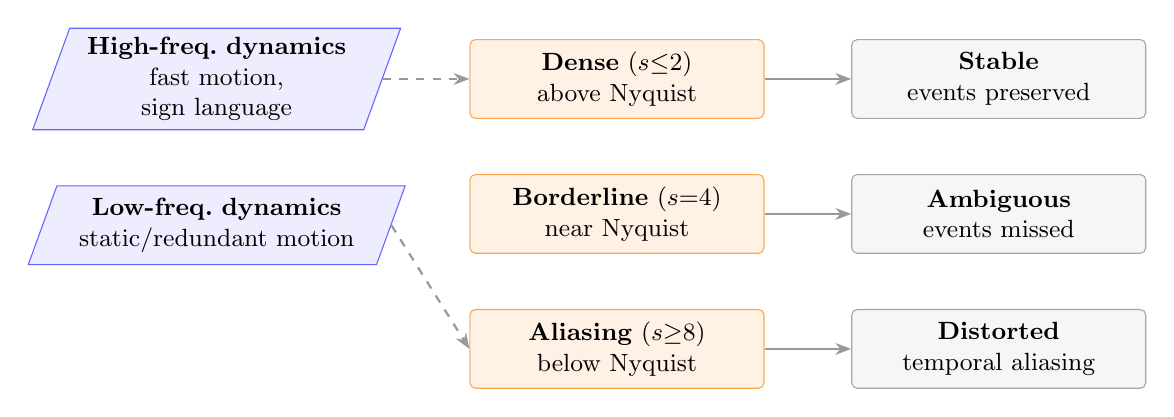
\begin{tikzpicture}[font=\small, node distance=7mm]
\tikzset{
  act/.style  ={draw, trapezium, trapezium left angle=70,
                trapezium right angle=110, align=center, minimum height=1.0cm, text width=3.5cm, fill=blue!7, draw=blue!60},
  samp/.style ={draw, rounded corners=2pt, align=center,
                minimum height=1.0cm, text width=3.5cm, fill=orange!10, draw=orange!70},
  obs/.style  ={draw, rounded corners=2pt, align=center,
                minimum height=1.0cm, text width=3.5cm, fill=gray!7, draw=gray!70},
  aI/.style={-{Stealth[length=2mm]},thick,dashed,draw=gray!80},
  aO/.style={-{Stealth[length=2mm]},thick,draw=gray!80}
}
\node (hf)[act]{\textbf{High-freq.\ dynamics}\\fast motion, sign language};
\node (lf)[act,below=of hf]{\textbf{Low-freq.\ dynamics}\\static/redundant motion};
\node (d)[samp,right=11mm of hf]{\textbf{Dense} ($s{\leq}2$)\\above Nyquist};
\node (n)[samp,below=of d]{\textbf{Borderline} ($s{=}4$)\\near Nyquist};
\node (a)[samp,below=of n]{\textbf{Aliasing} ($s{\geq}8$)\\below Nyquist};
\node (o1)[obs,right=11mm of d]{\textbf{Stable}\\events preserved};
\node (o2)[obs,below=of o1]{\textbf{Ambiguous}\\events missed};
\node (o3)[obs,below=of o2]{\textbf{Distorted}\\temporal aliasing};
\draw[aI](hf.east)--(d.west); \draw[aI](lf.east)--(a.west);
\draw[aO](d.east)--(o1.west); \draw[aO](n.east)--(o2.west); \draw[aO](a.east)--(o3.west);
\end{tikzpicture}
\end{adjustbox}
\caption{Temporal aliasing: high-frequency actions enter the distorted-evidence regime when sampling stride exceeds the Nyquist limit for that action class.}
\label{fig:aliasing_concept}
\end{figure}

\paragraph{Contributions.}
We conduct a systematic cross-architecture study of spatiotemporal aliasing:
\begin{enumerate}[leftmargin=*,topsep=2pt,itemsep=1pt]
\item \textbf{Temporal Demand Score (\TDS{})}: an architecture-averaged dataset
metric that consistently ranks 8 datasets by aliasing sensitivity, validated by leave-one-architecture-out analysis, architecture-family ablation (CNN-only, Transformer-only), and bootstrap confidence intervals (Sec.~\ref{sec:results_tds}; supplementary material). FineGym (55.9pp) rivals sign language (AUTSL, 53.0pp) as the highest-demand domain.
\item \textbf{Cross-architecture aliasing characterization}: 8,000 evaluation
configurations show that temporal aggregation design is a strong empirical correlate of aliasing behavior within our architecture pool, with VideoMamba and TimeSformer aliasing 3--5$\times$ less than CNNs and ViViT (Sec.~\ref{sec:results_temporal}).
\item \textbf{Target-resolution fine-tuning}: Fine-tuning each model at the deployment
resolution closes the cross-resolution gap by up to 39pp for CNNs while Transformers---already resolution-robust---require no retraining (Sec.~\ref{sec:results_spatial}).
\item \textbf{Measured inference latency}: GPU latency characterization
across all 8 models $\times$ 5 resolutions (bfloat16), enabling Nyquist-aware deployment budgeting per device class (Sec.~\ref{sec:results_latency}).
\item \textbf{Practical illustration and reproducibility package}: as a low-cost downstream use of the temporal-sweep results above---rather than a new routing algorithm in itself---a simple entropy-threshold router reduces average inference frames by 52\% while matching dense-sampling accuracy, outperforming FrameExit by $+4.2$pp under a matched-backbone comparison. We also provide an anonymized supplementary package containing the interactive dashboard, evaluation scripts, and result tables; the public dashboard and repository will be released after review (Sec.~\ref{sec:results_routing}).
\end{enumerate}

% =========================================================
\section{Related Work}
\label{sec:related}

\subsection{Video Recognition Architectures}

\textbf{CNN-based architectures.} 3D ConvNets learn spatiotemporal features end-to-end~\cite{tran2015c3d,carreira2017i3d}, while Non-local Networks introduce global self-attention~\cite{wang2018nonlocal}. Factorized variants such as R(2+1)D and MC3 improve optimization and efficiency~\cite{tran2018r2plus1d,tran2019video}; SlowFast processes two frame-rate streams simultaneously~\cite{feichtenhofer2019slowfast}.

\textbf{Transformer and SSM architectures.} Video Transformers extend patch-based recognition to time: TimeSformer uses divided space-time attention~\cite{bertasius2021timesformer}, ViViT uses factorized attention~\cite{arnab2021vivit}, and VideoMAE learns via masked patch reconstruction~\cite{tong2022videomae,wang2023videomaev2}. VideoMamba~\cite{li2024videomamba} brings selective state-space scanning~\cite{gu2023mamba,dao2024mamba2} to video. Prior robustness work benchmarks spatial and photometric corruptions~\cite{schiappa2023robustness}; we instead isolate temporal and spatial sampling effects across this architectural spectrum.

\subsection{Temporal Sampling and Adaptive Inference}

Efficient inference methods sample or process fewer frames. TSN and TSM define sparse-sampling recipes~\cite{wang2016tsn,lin2019tsm}; AdaFrame selects frames~\cite{wu2019adaframe}; AdaFocus crops regions~\cite{wang2021adafocus}; AR-Net adapts resolution~\cite{meng2020arnet}; and FrameExit uses confidence cascades~\cite{ghodrati2021frameexit}. Dataset-level temporal reasoning has been studied with shuffled frames~\cite{huang2018makes} and motion-only cues~\cite{sevilla2021only}. These works do not measure the accuracy cliff induced by controlled stride and coverage sweeps; our \TDS{} metric provides an architecture-averaged temporal-demand ranking.

\subsection{Sampling Theory in Deep Learning}

Sampling theory predicts that undersampling a signal below its highest temporal frequency creates aliasing~\cite{shannon1949communication}. Temporal aliasing is well documented in perception~\cite{vanrullen2007wagon}; in deep learning, strided operators can violate shift-invariance unless anti-aliased~\cite{zhang2019antialiased}. Frequency-domain analysis has been explored for action recognition~\cite{tran2014frequency}, but not as a large-scale cross-architecture stress test of modern video models.

% =========================================================
\section{Methodology}
\label{sec:method}

\begin{figure*}[t]
\centering
\resizebox{\textwidth}{!}{%
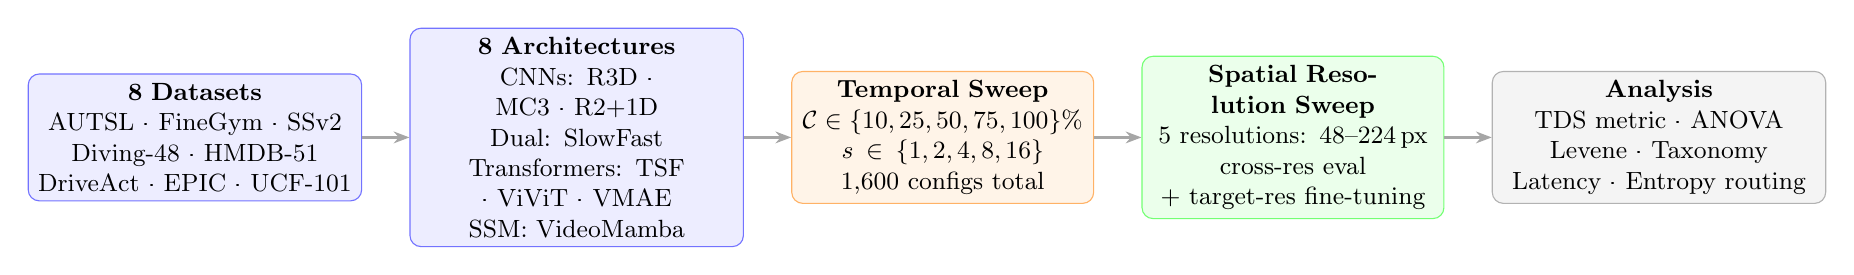
\begin{tikzpicture}[node distance=7mm,font=\small]
\tikzset{
  data/.style={draw,rounded corners,align=center,minimum height=8mm,text width=3.6cm,fill=blue!7,draw=blue!55},
  proc/.style={draw,rounded corners,align=center,minimum height=8mm,text width=3.6cm,fill=orange!9,draw=orange!60},
  p3/.style={draw,rounded corners,align=center,minimum height=8mm,text width=3.6cm,fill=green!8,draw=green!55},
  eval/.style={draw,rounded corners,align=center,minimum height=8mm,text width=4.0cm,fill=gray!9,draw=gray!60},
  arr/.style={-{Stealth[length=2mm]},thick,draw=gray!70}
}
\node(ds)[data,text width=4.0cm]{\textbf{8 Datasets}\\AUTSL · FineGym · SSv2\\Diving-48 · HMDB-51\\DriveAct · EPIC · UCF-101};
\node(ar)[data,right=6mm of ds,text width=4.0cm]{\textbf{8 Architectures}\\CNNs: R3D · MC3 · R2+1D\\Dual: SlowFast\\Transformers: TSF · ViViT · VMAE\\SSM: VideoMamba};
\node(e1)[proc,right=6mm of ar]{\textbf{Temporal Sweep}\\$\mathcal{C}\in\{10,25,50,75,100\}\%$\\$s\in\{1,2,4,8,16\}$\\1,600 configs total};
\node(e6)[p3,right=6mm of e1]{\textbf{Spatial Resolution Sweep}\\5 resolutions: 48--224\,px\\cross-res eval\\+ target-res fine-tuning};
\node(an)[eval,right=6mm of e6]{\textbf{Analysis}\\TDS metric · ANOVA\\Levene · Taxonomy\\Latency · Entropy routing};
\draw[arr](ds)--(ar); \draw[arr](ar)--(e1); \draw[arr](e1)--(e6); \draw[arr](e6)--(an);
\end{tikzpicture}}
\caption{Pipeline: 8 architectures evaluated across 8 datasets $\times$ 5 resolutions $\times$ 5 coverages $\times$ 5 strides = \textbf{8,000 configurations}. Temporal sweeps feed TDS, ANOVA, Levene, and entropy routing; spatial sweeps characterize cross-resolution robustness and target-resolution fine-tuning.}
\label{fig:pipeline}
\end{figure*}

\subsection{Datasets and Architectures}

Table~\ref{tab:datasets} summarizes the 8 datasets selected to span semantic domains, motion frequencies, and recording conditions. We evaluate 8 architectures from four families: (i) \textbf{3D CNNs}: R3D-18, MC3-18~\cite{tran2019video}, R(2+1)D-18~\cite{tran2018r2plus1d}; (ii) \textbf{dual-pathway}: SlowFast-R50~\cite{feichtenhofer2019slowfast}; (iii) \textbf{Transformers}: TimeSformer~\cite{bertasius2021timesformer}, ViViT~\cite{arnab2021vivit}, VideoMAE~\cite{tong2022videomae}; (iv) \textbf{SSM}: VideoMamba~\cite{li2024videomamba}. All models are fine-tuned from Kinetics-400 checkpoints using AdamW with cosine decay; learning rate $2\times10^{-5}$ (Transformers/SSMs) and $10^{-4}$ (CNNs).

\begin{table}[t]
\centering
\caption{\TDS{} = mean accuracy drop (stride=1$\to$16, cov=100\%) per Eq.~\ref{eq:tds}, averaged over all 8 architectures ($n{=}8$). Sorted by \TDS{}. \textbf{Bold} = the two co-equal highest-demand domains (their relative order is leave-one-out sensitive; ranks 3--8 are stable under the supplementary robustness analysis).}
\label{tab:datasets}
\scriptsize\tabtight
\begin{tabular}{l r r l r r}
\toprule
Dataset & Classes & Videos & Domain & \TDS{} & $n$ \\
\midrule
FineGym~\cite{shao2020finegym}       &  97 & 1,960 & Fine-grained sport & \textbf{55.9pp} & 8 \\
AUTSL~\cite{sincan2020autsl}         & 226 & 4,418 & Sign language      & \textbf{53.0pp} & 8 \\
SSv2~\cite{goyal2017ssv2}            & 174 & 3,464 & Causal/temporal    & 27.6pp          & 8 \\
DriveAct~\cite{martin2019driveact}   &  33 &   448 & In-vehicle         & 21.9pp          & 8 \\
Diving-48~\cite{li2018diving48}      &  48 &   743 & Fine-grained       & 19.2pp          & 8 \\
HMDB-51~\cite{kuehne2011hmdb}        &  51 &   885 & Sports             & 16.6pp          & 8 \\
EPIC-Kitchens~\cite{damen2022epic}   &  89 & 1,020 & Egocentric         &  9.7pp          & 8 \\
UCF-101~\cite{soomro2012ucf101}      & 101 & 2,020 & Appearance         &  4.9pp          & 8 \\
\bottomrule
\end{tabular}
\end{table}

\subsection{Temporal Sampling Protocol}

We decouple \textit{temporal coverage} $\mathcal{C}$ (fraction of clip observed) from \textit{temporal stride} $s$ (sampling density), forming a 5$\times$5 grid: $\mathcal{C}\in\{10,25,50,75,100\}\%$ and $s\in\{1,2,4,8,16\}$. The temporal sweep at native resolution yields $8{\times}8{\times}25{=}\mathbf{1{,}600}$ model--dataset--configuration triples (each evaluated over ${\approx}20$ clips per class). Combined with the spatial resolution sweep (5 resolutions), the total reaches \textbf{8,000 evaluation configurations}.

\paragraph{Coverage implementation.}
Coverage is applied from the \emph{beginning} of each clip: the first $\lfloor T\cdot\mathcal{C}/100\rfloor$ frames form the candidate pool, and $s$ controls sampling density within that window. This simulates a sensor that observes only a leading fraction of the action and gives the sharpest measurement of how early the model has enough temporal context. Random window placement would confound temporal structure with missing-data effects; a 10\% random-window check on SSv2 gives qualitatively similar coverage effects (supplementary material).

\subsection{Spatial Resolution Protocol}

\paragraph{Cross-resolution evaluation.}
We evaluate all 8 native-resolution checkpoints on all 8 datasets at 48, 96, 112, 160, 224, and 336\,px without retraining, measuring accuracy retention when the input resolution differs from the native training resolution (112px for CNNs, 224px for Transformers and VideoMamba).

\paragraph{Target-resolution fine-tuning.}
For each model--dataset--resolution triple at 48--224\,px, we fine-tune from the native-resolution checkpoint for 10 additional epochs. For Transformers and VideoMamba, positional embeddings are bicubically interpolated from the native grid to the target grid before fine-tuning; discarding mismatched positional embeddings causes a large accuracy cliff. CNNs transfer directly, and SlowFast uses adaptive average pooling to support non-native resolutions.

\subsection{Temporal Demand Score (\texorpdfstring{\TDS{}}{TDS})}

We define \TDS{} as the architecture-averaged accuracy drop from stride=1 to stride=16:
\begin{equation}
  \TDS(\mathcal{D}) = \frac{1}{|\mathcal{M}|} \sum_{m\in\mathcal{M}} \bigl[\mathrm{Acc}(m,\mathcal{D},s{=}1) - \mathrm{Acc}(m,\mathcal{D},s{=}16)\bigr]^+
  \label{eq:tds}
\end{equation}
where $[\cdot]^+$ excludes feature-collapsed models. \TDS{} is architecture-pool averaged, but its dataset ranking is stable under leave-one-architecture-out, family ablations, and bootstrap resampling over our 8-model pool (Sec.~\ref{sec:results_tds}; supplementary material), suggesting it reflects dataset temporal structure rather than any single model.

\subsection{Statistical Analysis}

For each model-dataset pair, two-way ANOVA decomposes accuracy variance into coverage and stride components (effect size $\eta^2$). Levene's test detects per-class variance inflation under sparse sampling. Post-hoc Welch tests with Bonferroni correction identify aliasing cliffs.

\subsection{Entropy-Based Routing}

Given temporal-sweep results at two operating points---cheap: cov=100\%/$s$=4 (4 effective frames); dense: cov=100\%/$s$=1 (16 frames)---we route video $v$ by threshold: \[ \hat{y}(v) = \begin{cases}
    \hat{y}_\text{cheap} & \text{if } \max_c\,p(c\mid v,s{=}4) > \tau \\
    \hat{y}_\text{dense} & \text{otherwise}
  \end{cases}
\] We sweep $\tau\in[0.10,\,0.95]$ and report the Pareto-optimal point at avg frames~$\leq8$. No retraining is required; only the existing temporal-sweep inference is reused.

% =========================================================
\section{Results}
\label{sec:results}

\subsection{Temporal Demand Score Validates Architecture-Independent Ranking}
\label{sec:results_tds}

Figure~\ref{fig:tds_spectral} (left) ranks datasets by \TDS{}. \textbf{FineGym (55.9pp)} is the most important new finding in this dimension: fine-grained gymnastics phase transitions rival AUTSL sign language (53.0pp), showing that sport is not inherently low-\TDS{} when the label space requires sub-second phase discrimination. AUTSL requires dense sampling to discriminate fine handshape transitions, but FineGym's phase boundaries are comparably demanding. UCF-101 (4.9pp) is nearly appearance-driven: object identity and static scene cues often suffice.

Crucially, ranks 3--8 are stable under leave-one-architecture-out: removing any single architecture leaves SSv2, DriveAct, Diving-48, HMDB-51, EPIC-Kitchens, and UCF-101 in the same order. Only the \#1/\#2 position swaps when VideoMamba is removed, so we report FineGym and AUTSL as co-equal high-\TDS{} domains. This stability also holds for CNN-only, Transformer-only, and Transformer+SSM pools (Spearman $\rho\geq0.976$ against the full pool), while bootstrap resampling gives a FineGym$-$AUTSL 95\% CI of $[-4.6,\,+11.7]$pp, consistent with zero (supplementary material).

\paragraph{Spectral validation.}
Figure~\ref{fig:tds_spectral} (right) correlates optical-flow magnitude with per-class aliasing loss. AUTSL and DriveAct show the expected positive within-dataset trend: classes with more motion alias more. EPIC-Kitchens is near zero, suggesting that egocentric camera motion decouples raw flow from action-relevant demand. FineGym is inverted ($r=-0.475$, $p<0.0001$): high-flow gymnastics classes often remain visually distinctive from almost any frame, while low-flow held positions or balance corrections depend on brief key moments. Thus raw flow magnitude is only a partial proxy for temporal demand, especially when class identity hinges on a discrete event rather than sustained motion (Table~\ref{tab:spectral}).

\paragraph{The inversion generalizes beyond FineGym.} A direct spectral test on all 8 datasets across 5 resolutions pairs whole-frame optical-flow cutoff frequency with empirical stride-sensitivity at the same resolution (40 points; supplementary material). The relationship is significantly \emph{negative} ($\rho=-0.63$, $p=1.1{\times}10^{-5}$): UCF-101 and HMDB-51 have high flow-derived cutoffs but low stride-sensitivity, while FineGym and AUTSL have the highest stride-sensitivity at lower cutoff frequencies. Thus whole-frame flow does not literally validate the Nyquist analogy; it mainly shows that classifier-relevant temporal evidence is often localized and diluted by bulk motion. When temporal demand is instead measured directly in label space---via the temporal concentration of the model's correct-class confidence under a sliding window, rather than bulk pixel flow---the expected positive relationship is recovered: across all 8 datasets, per-class confidence concentration is positively associated with per-class aliasing loss (pooled Spearman $\rho=+0.26$ over a 6-architecture ensemble, positive in 8/8 datasets, significant in 4; supplementary material).

\begin{figure}[t]
  \centering
  \includegraphics[width=\columnwidth]{images/main_fig3_tds_spectral.pdf}
  \caption{\textbf{Left}: \TDS{} ranking---mean accuracy drop from stride=1 to 16 averaged over all 8 architectures ($n{=}8$). FineGym (55.9pp) and AUTSL (53.0pp) are co-equal highest-demand domains (order between them is leave-one-out sensitive; see supplementary material); UCF-101 (4.9pp) is appearance-dominated. Positions 3--8 are exactly stable under leave-one-architecture-out. \textbf{Right}: Pearson correlation between optical-flow magnitude and per-class aliasing loss (8 datasets). AUTSL and DriveAct show the expected positive correlation; EPIC-Kitchens is near-zero (background camera motion confounds flow); FineGym shows the strongest correlation of any dataset but in the opposite direction ($r=-0.475$): discrete-event classes alias more than sustained-motion ones.}
  \label{fig:tds_spectral}
\end{figure}

\begin{table}[t]
\centering
\caption{Spectral validation: Pearson $r$ between optical-flow magnitude and per-class aliasing loss. Flow alone partially explains temporal demand; camera-motion-heavy datasets (EPIC, UCF) show weak correlation.}
\label{tab:spectral}
\scriptsize\tabtight
\begin{tabular}{l r r c r}
\toprule
Dataset & Classes & Pearson $r$ & Significant & Interpretation \\
\midrule
FineGym       &  97 & $-0.475$ & \checkmark & Discrete-event classes alias more \\
DriveAct      &  33 & 0.327 & marginal   & Flow $\sim$ arm motion \\
AUTSL         & 226 & 0.285 & \checkmark & Flow $\sim$ hand speed \\
SSv2          & 174 & 0.184 & \checkmark & Causal/object motion \\
HMDB-51       &  51 & 0.180 & $\times$   & Mixed motion types \\
Diving-48     &  47 & 0.140 & $\times$   & Body rotation dominated \\
UCF-101       & 101 & 0.031 & $\times$   & Appearance dominates \\
EPIC-Kitchens &  89 & $-0.002$& $\times$ & Camera motion confounds \\
\bottomrule
\end{tabular}
\end{table}

\subsection{Cross-Architecture Temporal Aliasing}
\label{sec:results_temporal}

\paragraph{Attention type correlates with aliasing.}
Table~\ref{tab:e1_full} shows stride=1 accuracy and stride=16 drop. The central observational finding is that aliasing tracks temporal aggregation design more closely than broad architecture family in this pool. The robust group is TimeSformer (divided attention, 10.3pp mean drop) and VideoMamba (SSM, 11.4pp). Both preserve global temporal context under aggressive subsampling: TimeSformer via full-clip cross-frame attention, and VideoMamba via recurrent state accumulation.

VideoMamba's robustness is markedly \emph{bimodal}. It drops only 4.0pp on average over UCF-101, HMDB-51, EPIC-Kitchens, Diving-48, and DriveAct, which would make it the most robust model by a large margin if these were the only domains considered. But on the three highest-\TDS{} domains, VideoMamba suffers substantially: FineGym (40.8pp), AUTSL (16.0pp), and SSv2 (14.1pp). FineGym most clearly inverts the SSM-vs-Transformer ranking: TimeSformer drops 36.1pp vs.\ VideoMamba's 40.8pp, a 4.7pp gap favoring divided attention. The same direction holds on SSv2, while AUTSL is tied. We hypothesize that VideoMamba's running state smooths over high-frequency phase transitions, whereas TimeSformer can selectively attend to the most discriminative frames.

The SSv2 result extends beyond temporal frequency: SSv2 tests causal ordering (e.g., move object left then right), not just temporal density. SSM recurrence over skipped frames integrates corrupted order evidence, while appearance-driven UCF-101 remains stable. The fragile group comprises SlowFast (42.1pp), VideoMAE (32.8pp), ViViT (30.0pp), R2+1D (30.0pp), R3D-18 (29.7pp), and MC3-18 (22.6pp). ViViT is the key anomaly: a Transformer whose factorized attention remains vulnerable to frame dropout.

\begin{figure*}[t]
  \centering
  \includegraphics[width=\textwidth]{images/main_fig1_aliasing_curves.pdf}
  \caption{Accuracy vs.\ stride (cov=100\%) for three representative datasets. \textbf{AUTSL} (\TDS{}=53.0pp): TimeSformer and VideoMamba remain most stable; all other models cliff above stride=4. \textbf{SSv2} (\TDS{}=27.6pp): clear two-tier separation between robust (TSF, VMamba) and fragile models. \textbf{UCF-101} (\TDS{}=4.9pp): minimal sensitivity across all architectures. These three datasets cover the full \TDS{} range, validating the metric.}
  \label{fig:aliasing_curves}
\end{figure*}

\begin{table*}[t]
\centering
\caption{Full temporal aliasing table: stride=1 accuracy (\%) / drop at stride=16 (pp), cov=100\%. Rows sorted by average drop across all 8 datasets.}
\label{tab:e1_full}
\scriptsize\tabtight
\begin{adjustbox}{max width=\textwidth}
\begin{tabular}{l @{\hskip4pt} cccccccc @{\hskip4pt} r}
\toprule
Model (family) & UCF-101 & SSv2 & HMDB-51 & Diving-48 & FineGym & AUTSL & DriveAct & EPIC-Kit. & Avg drop \\
\midrule
TimeSformer (div.\ attn) & 91.0/0.0 & 42.3/12.8 & 79.9/4.0 & 38.2/2.0 & 66.4/36.1 & 66.8/16.0 & 67.6/8.5 & 32.3/2.9 & \textbf{10.3pp} \\
VideoMamba (SSM)         & 88.4/\textcolor{teal}{+0.8} & 43.9/14.1 & 69.8/3.6 & 36.5/4.9 & 72.7/40.8 & 65.6/16.0 & 57.6/9.6 & 28.3/1.2 & \textbf{11.4pp} \\
\midrule
MC3-18 (CNN-mix)  & 85.4/2.9  & 33.6/26.7 & 78.6/9.7  & 31.6/12.4 & 64.2/51.1 & 63.7/55.5 & 69.0/13.8 & 36.2/8.6  & 22.6pp \\
R3D-18 (CNN-3D)   & 81.2/6.0  & 37.1/28.2 & 80.3/21.1 & 28.8/16.0 & 71.5/61.4 & 75.0/68.5 & 68.3/23.9 & 37.2/12.7 & 29.7pp \\
R2+1D (CNN-sep.)  & 88.6/5.1  & 42.6/30.7 & 73.1/17.6 & 35.3/18.8 & 76.8/64.2 & 75.9/67.2 & 62.5/24.8 & 35.5/11.7 & 30.0pp \\
ViViT (fact.\ attn) & 94.3/5.2 & 38.3/30.6 & 80.2/19.4 & 53.0/36.3 & 69.9/55.2 & 74.6/62.1 & 67.4/20.3 & 32.9/11.1 & 30.0pp \\
VideoMAE (MAE)    & 95.4/3.5  & 52.4/34.4 & 84.0/20.2 & 48.6/23.4 & 78.0/67.8 & 79.6/61.2 & 73.9/40.8 & 37.7/10.8 & 32.8pp \\
SlowFast (dual)   & 87.6/15.4 & 49.5/43.0 & 79.3/37.4 & 50.5/39.7 & 78.2/71.5 & 82.3/77.6 & 72.5/33.7 & 39.4/18.5 & \textbf{42.1pp} \\
\bottomrule
\end{tabular}
\end{adjustbox}
\end{table*}

\paragraph{Architecture-specific failure modes.}
SlowFast cliffs at stride 2$\to$4 because its fast and slow pathways are simultaneously starved; on FineGym it has the best base accuracy (78.2\%) but the largest drop (71.5pp). VideoMAE is spatially strong but temporally fragile: masked patch reconstruction does not train robustness to missing frames. VideoMamba's failures concentrate on high-frequency phase changes (FineGym), handshape transitions (AUTSL), and ordering-sensitive interactions (SSv2).

\paragraph{Cross-architecture sensitivity heatmap.}
Figure~\ref{fig:heatmap} shows the full coverage$\times$stride sensitivity matrix averaged over 8 datasets, with models sorted by mean \TDS{}. The diagonal structure---robust models maintaining a flat plateau while fragile models show sharp gradients along the stride axis---is consistent across datasets (full per-model, per-dataset heatmaps are in the supplementary material).

\begin{figure*}[t]
  \centering
  \includegraphics[width=\textwidth]{images/main_fig2_aliasing_heatmap.pdf}
  \caption{Cross-architecture sensitivity heatmap: accuracy (\%) averaged over 8 datasets across the coverage$\times$stride grid. Models sorted left-to-right by mean aliasing robustness. VideoMamba and TimeSformer maintain a flat high-accuracy plateau; SlowFast and ViViT show dramatic stride-driven collapse (red gradient).}
  \label{fig:heatmap}
\end{figure*}

\subsection{Statistical Validation (ANOVA and Levene's Test)}
\label{sec:stats}

\paragraph{Effect sizes.}
Table~\ref{tab:anova} reports two-way ANOVA $\eta^2$ values (mean$\pm$std over 8 datasets). Coverage is the dominant factor across all models ($\eta^2_\text{cov}=0.53$--$0.90$). Stride effect size distinguishes the two groups: VideoMamba and TimeSformer have $\eta^2_\text{stride}\approx0.08$, while SlowFast reaches $0.35$---a 4.4$\times$ difference confirming that stride is architecturally consequential for fragile models. Full per-dataset $\eta^2$ tables are provided in the supplementary material.

\begin{table}[t]
\centering
\caption{ANOVA effect sizes ($\eta^2$, mean$\pm$std over 8 datasets). All stride effects significant ($p{<}0.05$). Coverage dominates; stride separates robust from fragile.}
\label{tab:anova}
\scriptsize\tabtight
\begin{tabular}{l cc c}
\toprule
Model & $\eta^2_\text{stride}$ & $\eta^2_\text{cov}$ & Interpretation \\
\midrule
VideoMamba     & $0.09 \pm 0.14$ & $0.88 \pm 0.07$ & Robust \\
TimeSformer    & $0.11 \pm 0.13$ & $0.88 \pm 0.06$ & Robust \\
MC3-18         & $0.20 \pm 0.07$ & $0.73 \pm 0.10$ & Moderate \\
R2+1D          & $0.23 \pm 0.08$ & $0.69 \pm 0.09$ & Fragile \\
R3D-18         & $0.24 \pm 0.06$ & $0.68 \pm 0.07$ & Fragile \\
VideoMAE       & $0.20 \pm 0.11$ & $0.73 \pm 0.14$ & Moderate \\
ViViT          & $0.26 \pm 0.05$ & $0.65 \pm 0.09$ & Fragile \\
SlowFast       & $0.35 \pm 0.07$ & $0.53 \pm 0.09$ & Most fragile \\
\bottomrule
\end{tabular}
\end{table}

\paragraph{Variance inflation.}
Levene's test shows significant inter-class variance inflation in 67\% of model-dataset pairs ($p<0.05$, Bonferroni-corrected across all 64 model$\times$dataset comparisons). The worst cases are VideoMAE/HMDB-51 ($2.0\times$) and R3D-18/HMDB-51 ($1.85\times$), while TimeSformer and VideoMamba remain stable ($\approx1.1\times$). Thus sparse sampling can create class-specific failures that mean accuracy hides.

\subsection{Action Sensitivity Taxonomy}
\label{sec:taxonomy}

We classify each action class into three tiers by per-class aliasing loss (accuracy drop, stride=1$\to$16). Tier boundaries use the 33rd/67th percentiles.

\textbf{High-sensitivity} actions are temporally critical: in AUTSL, even the Low tier loses 38pp, confirming that the entire dataset requires dense sampling. In contrast, the UCF-101 Low tier loses only 0.3pp: static, appearance-driven actions are virtually unaffected. Table~\ref{tab:taxonomy_thresholds} reports per-dataset tier boundaries. AUTSL's Low threshold starts at 66.9pp, above the High threshold of any other dataset, confirming that sign language forms a distinct temporal-frequency regime.

\begin{table}[t]
\centering
\caption{Taxonomy tier boundaries (accuracy drop pp): classes below Low threshold alias minimally; above High threshold alias severely. Computed at cov=100\%, stride=1$\to$16.}
\label{tab:taxonomy_thresholds}
\scriptsize\tabtight
\begin{tabular}{l r r r r}
\toprule
Dataset & Low $\leq$ & High $>$ & \# High & \# Low \\
\midrule
AUTSL         & 66.9pp & 73.9pp & 75 & 74 \\
Diving-48     & 25.0pp & 47.7pp & 16 & 16 \\
SSv2          & 59.7pp & 76.9pp & 58 & 57 \\
HMDB-51       &  8.4pp & 28.5pp & 17 & 17 \\
EPIC-Kitchens &  0.0pp & 19.4pp & 30 & 11 \\
DriveAct      & 14.8pp & 51.0pp & 11 & 11 \\
UCF-101       &  1.4pp &  7.5pp & 35 & 31 \\
\bottomrule
\end{tabular}
\end{table}

\textbf{Clip duration effect.} Counter-intuitively, shorter clips alias more severely (Pearson $r=-0.3$ to $-0.8$ across models): short clips have less temporal redundancy, so each missed frame removes a larger fraction of available evidence. On UCF-101, clips $>$6s lose only 1.5pp at stride=16 vs.\ 16.2pp for clips $<$3s. This suggests that short clips should receive dense sampling irrespective of model confidence (details in the supplementary material).

\subsection{Spatial Resolution and Target-Resolution Fine-Tuning}
\label{sec:results_spatial}

\paragraph{Cross-resolution robustness.}
Figure~\ref{fig:spatial} and Table~\ref{tab:spatial} show accuracy vs.\ input resolution for all 8 models on SSv2, evaluated \emph{without retraining}. The same attention-type split observed in the temporal domain reappears here. CNNs (native 112px) degrade sharply at higher resolutions: R2+1D drops from 42.6\% at 112px to 5.9\% at 336px ($-36.6$pp). Transformers and VideoMamba (native 224px) stay within $\pm$7pp across 96--336px.

\begin{figure}[t]
  \centering
  \includegraphics[width=\columnwidth]{images/main_fig5_spatial_resolution.pdf}
  \caption{Accuracy vs.\ input resolution on SSv2 (no retraining). CNNs (dashed, native=112px) degrade severely at higher resolutions; Transformers and VideoMamba (solid, native=224px) stay within $\pm$7pp across 96--336px. Filled markers denote each model's native training resolution.}
  \label{fig:spatial}
\end{figure}

\begin{table}[t]
\centering
\caption{Spatial robustness on SSv2 (no retraining). Bold = native resolution. $\Delta_\text{max}$ = largest drop from native.}
\label{tab:spatial}
\scriptsize\tabtight
\begin{adjustbox}{max width=\columnwidth}
\begin{tabular}{l r rrrrr r}
\toprule
Model & Native & 96px & 112px & 160px & 224px & 336px & $\Delta_\text{max}$ \\
\midrule
R3D-18      & 112px & 35.9 & \textbf{37.1} & 30.3 & 17.2 &  5.8 & $-31.4$pp \\
MC3-18      & 112px & 32.4 & \textbf{33.6} & 27.8 & 14.8 &  4.4 & $-29.2$pp \\
R2+1D       & 112px & 40.1 & \textbf{42.6} & 36.2 & 20.8 &  5.9 & $-36.6$pp \\
SlowFast    & 224px & 27.7 & 32.4 & 45.7 & \textbf{49.5} & 36.0 & $-21.8$pp \\
\midrule
TimeSformer & 224px & 39.3 & 39.4 & 41.4 & \textbf{42.3} & 42.1 & $-3.0$pp \\
ViViT       & 224px & 36.4 & 37.1 & 38.1 & \textbf{38.3} & 38.0 & $-1.9$pp \\
VideoMAE    & 224px & 48.9 & 49.2 & 51.5 & \textbf{52.3} & 51.9 & $-3.4$pp \\
VideoMamba  & 224px & 37.5 & 39.3 & 42.5 & \textbf{43.9} & 43.8 & $-6.4$pp \\
\bottomrule
\end{tabular}
\end{adjustbox}
\end{table}

The CNN/Transformer split holds across all 8 datasets (supplementary material). On AUTSL, R3D-18 drops from 75.0\% to 2.0\% at 336px ($-73.0$pp), whereas Transformers remain within $\pm$8pp on 7 of 8 datasets; EPIC-Kitchens is the main exception.

\paragraph{Target-resolution fine-tuning recovers CNN performance.}
Table~\ref{tab:p3} shows family-level averages after target-resolution tuning. CNNs recover sharply: at 224px, cross-resolution accuracy is 30.0\%, but fine-tuning reaches 69.2\% ($+39.2$pp). Transformers improve modestly because they are already robust across resolutions.

\begin{table}[t]
\centering
\caption{Target-resolution fine-tuning: family-level mean accuracy (\%) averaged over all 8 datasets, after fine-tuning from the native-resolution checkpoint for 10 epochs at each target spatial resolution. CNNs benefit by up to 39.2pp at off-native resolutions. Transformers already achieve near-native accuracy without retraining.}
\label{tab:p3}
\scriptsize\tabtight
\begin{tabular}{l ccccc}
\toprule
Family & 48px & 96px & 112px & 160px & 224px \\
\midrule
CNN (3 models)  & 49.3 & 64.9 & 67.7 & 68.5 & 69.2 \\
Transformer (3) & 36.6 & 56.3 & 60.3 & 66.9 & 71.4 \\
SSM (VideoMamba) & 31.5 & 41.2 & 45.1 & 54.5 & 59.7 \\
Dual-CNN (SlowFast) & 36.2 & 73.3 & 71.9 & 71.6 & 67.5 \\
\bottomrule
\end{tabular}
\end{table}

\subsection{Inference Latency and Deployment Budgeting}
\label{sec:results_latency}

Table~\ref{tab:latency} reports measured bfloat16 latency at batch 1. VideoMamba is slowest (8--15ms), 4--8$\times$ slower than VideoMAE (1.6--2.8ms) despite its SSM design. VideoMAE gives the best Transformer accuracy per ms, while CNN latency scales predictably with resolution.

\begin{table}[t]
\centering
\caption{Inference latency (ms/clip, bfloat16, batch=1, RTX PRO 6000 Blackwell). VideoMamba is 4--8$\times$ slower than VideoMAE despite being an SSM. Scale to other devices: RTX 4090 $\times$1.5, Jetson AGX Orin $\times$10, Jetson Nano $\times$50.}
\label{tab:latency}
\scriptsize\tabtight
\begin{tabular}{l ccccc}
\toprule
Model & 48px & 96px & 112px & 160px & 224px \\
\midrule
R3D-18      & 0.61 & 0.89 & 1.20 & 1.76 & 2.78 \\
MC3-18      & 0.61 & 0.85 & 1.18 & 1.84 & 3.15 \\
R2+1D       & 1.39 & 2.21 & 2.54 & 4.10 & 5.77 \\
SlowFast    & 3.09 & 3.11 & 3.11 & 3.13 & 4.10 \\
\midrule
TimeSformer & 3.25 & 3.24 & 3.20 & 3.20 & 4.30 \\
ViViT       & 1.55 & 1.77 & 1.99 & 3.19 & 6.35 \\
VideoMAE    & 1.57 & 1.79 & 1.78 & 1.92 & 2.82 \\
VideoMamba  & 8.06 & 8.15 & 8.18 & 10.03 & 15.44 \\
\bottomrule
\end{tabular}
\end{table}

\subsection{Entropy-Based Adaptive Routing}
\label{sec:results_routing}

Table~\ref{tab:routing} compares entropy routing at average frame budget $\leq8$ (full curves in the supplementary material). Thresholds are swept on the validation split to trace the achievable Pareto frontier; we treat the router as a deployment illustration rather than a separately trained method. AdaFocus~\cite{wang2021adafocus} and AR-Net~\cite{meng2020arnet} use ResNet-50 and are informational. The controlled comparison is FrameExit~\cite{ghodrati2021frameexit}, also on TimeSformer: entropy routing reaches 42.5\% vs.\ 38.4\% ($+4.2$pp) with fewer frames (7.7 vs.\ 9.9).

\begin{figure}[t]
  \centering
  \includegraphics[width=0.82\textwidth]{images/main_fig4_routing_comparison.pdf}
  \caption{Entropy routing on SSv2: accuracy vs.\ average frames as $\tau$ sweeps between 4-frame cheap and 16-frame dense inference.}
  \label{fig:routing}
\end{figure}

\begin{table}[t]
\centering
\caption{Routing comparison on SSv2 at avg $\leq$8 frames. The fair, same-backbone comparison is Entropy (ours) vs.\ FrameExit, both on TimeSformer. AdaFocus/AR-Net use a different backbone (ResNet-50) and are reported only as context for absolute numbers reported in their respective papers, not as a controlled comparison.}
\label{tab:routing}
\scriptsize\tabtight
\begin{tabular}{l c c c}
\toprule
Method & Avg frames & SSv2 Top-1 & Backbone \\
\midrule
\multicolumn{4}{l}{\textit{Informational only: different backbone}} \\
AdaFocus~\cite{wang2021adafocus} & 8.0 & 54.7\% & ResNet-50 \\
AR-Net~\cite{meng2020arnet}      & 8.0 & 48.6\% & ResNet-50 \\
\midrule
\multicolumn{4}{l}{\textit{Controlled comparison: same TimeSformer backbone}} \\
Oracle upper bound      & 7.7  & 47.3\% & TimeSformer \\
Fixed 16f (dense)       & 16.0 & 42.3\% & TimeSformer \\
Fixed 8f                & 8.0  & 42.3\% & TimeSformer \\
\textbf{Entropy (ours)} & \textbf{7.7} & \textbf{42.5\%} & TimeSformer \\
Fixed 4f (cheap)        & 4.0  & 41.5\% & TimeSformer \\
FrameExit~\cite{ghodrati2021frameexit} & 9.9 & 38.4\% & TimeSformer \\
\bottomrule
\end{tabular}
\end{table}

Across model-dataset pairs, 77\% of videos route to cheap 4-frame inference on average. VideoMAE gives the highest absolute routed accuracy, while TimeSformer achieves the highest cheap-routing rates on temporal-critical datasets.

% =========================================================
\section{Discussion}
\label{sec:discussion}

\paragraph{Architecture and sampling.}
The robust temporal group combines global divided attention (TimeSformer) or recurrent state integration (VideoMamba), while the fragile group includes CNNs and factorized-attention Transformers. VideoMamba remains bimodal: it is nearly flat on low-\TDS{} datasets but still aliases on FineGym, AUTSL, and SSv2, where brief phase changes, handshape transitions, or causal order matter. Spatial robustness follows a related but distinct pattern: patch-token Transformers are resolution-stable, whereas CNNs require target-resolution fine-tuning; ViViT's spatial robustness despite temporal fragility separates tokenization effects from temporal aggregation effects.

\paragraph{Spatial robustness.}
The spatial results suggest that temporal and spatial robustness share some architectural ingredients but are not identical. CNNs' strided filters are tied to the spatial scale seen during training, which explains the sharp off-resolution degradation and the large recovery from target-resolution fine-tuning. Transformers remain stable across most resolutions because patch tokenization and global aggregation tolerate scale shifts, yet ViViT shows that this spatial invariance does not guarantee temporal robustness. VideoMamba again sits between these regimes: stable on some datasets, but less reliable on cluttered egocentric or in-vehicle scenes.

\paragraph{Deployment implications.}
Resolution, latency, and sampling density should be searched jointly rather than treated as independent knobs. High-\TDS{} domains require stride$\leq$2, moderate-\TDS{} domains tolerate stride$\leq$4, and low-\TDS{} domains tolerate stride up to 16. Target-resolution tuning makes CNN resolution a cost dial; TimeSformer routing at 7.7 frames matches dense R2+1D on SSv2. These trade-offs are deployment-relevant because a model that is slightly less accurate at dense sampling can become preferable once resolution, stride, and hardware latency are optimized together.

This also changes how one should read fixed-recipe video benchmarks. A single native-resolution, fixed-stride number can hide the fact that two models exchange rank once the temporal budget or input resolution changes. The dashboard and tables therefore expose operating points rather than only peak accuracy, making the sampling constraint explicit.

\paragraph{Limitations.}
Our architecture analysis is observational: temporal aggregation design covaries with tokenization, pretraining objective, capacity, and optimization recipe, so we report empirical associations rather than a controlled causal mechanism. A stronger test would swap temporal modules inside a shared backbone while holding training and capacity fixed. The Nyquist framing is best supported in label space: whole-frame flow is inversely related to stride-sensitivity, but temporal concentration of correct-class confidence is positively associated with per-class aliasing (pooled Spearman $\rho=+0.26$; supplementary material). Routing thresholds trace validation Pareto frontiers and should be calibrated on a held-out split before deployment.

% =========================================================
\section{Conclusion}
\label{sec:conclusion}

We presented a large-scale cross-architecture study of spatiotemporal aliasing in video action recognition. Across 8 architectures, 8 datasets, and 8,000 configurations, aliasing tracks temporal aggregation design more than broad model family, with ViViT showing that Transformers are not automatically temporally robust. The \TDS{} metric identifies FineGym and AUTSL as co-equal high-demand domains, establishing fine-grained sport as a high-aliasing regime. VideoMamba is robust but bimodal and slow on GPU; target-resolution fine-tuning closes the CNN resolution gap by up to 39pp; and entropy routing cuts inference cost by 52\% without accuracy loss on the validation Pareto frontier. 

\bibliographystyle{splncs04}
\bibliography{main}

\end{document}
